% This is samplepaper.tex, a sample chapter demonstrating the
% LLNCS macro package for Springer Computer Science proceedings;
% Version 2.20 of 2017/10/04
%
\documentclass[runningheads]{llncs}
%
\usepackage{graphicx}
\usepackage{tabularx}
\usepackage{pgfplots}
\usepgfplotslibrary{external}

\pgfplotsset{width=\textwidth,compat=1.9}
% Used for displaying a sample figure. If possible, figure files should
% be included in EPS format.
%
% If you use the hyperref package, please uncomment the following line
% to display URLs in blue roman font according to Springer's eBook style:
% \renewcommand\UrlFont{\color{blue}\rmfamily}

\begin{document}
%
\title{Building a Knowledge Graph}
%
\titlerunning{BKG}
% If the paper title is too long for the running head, you can set
% an abbreviated paper title here
%

\newcolumntype{Y}{>{\centering\arraybackslash}X}
\author{Lukas Bl{\"u}baum \and Nick D{\"u}sterhus \and Monika Werner}
%
\authorrunning{L. Bl{\"u}baum,Nick D{\"u}sterhus  et al.}
% First names are abbreviated in the running head.
% If there are more than two authors, 'et al.' is used.
%
\institute{University of Paderborn, Padeborn 33098, Germany \\
%\email{lncs@springer.com}\\ 
\email{\{lukasbl,nduester,mwerner\}@uni-paderborn.de} \\
\url{https://github.com/LukasBluebaum/BKG} 
% ABC Institute, Rupert-Karls-University Heidelberg, Heidelberg, Germany\\
%\email{\{abc,lncs\}@uni-heidelberg.de}
}
%
\maketitle              % typeset the header of the contribution
%
\begin{abstract}
The goal of this proseminar was to create an encyclopetic knowledge graph from a large text corpus like a wikipedia dump. In order to learn and better understand the basics of Semantic Web technologies. For this we were given a wikipedia dump and the core ontology of DBpedia. To facilitate this task we were introduced to several tools including FOX and DBpedia Spotlight \cite{spotlight}. The whole project is written in Java and as license we used the GNU General Public License v3.0. The documented source code, including instructions on how to run the code, can be found on the given Github repository.

\keywords{Knowledge Graphs  \and Semantic Web \and Coreference Resolution \and Named Entity Recognition
\and Entity Disambiguation \and Relation Extraction \and Fox \and Spotlight }
\end{abstract}


\section{Introduction}
Websites like Wikipedia contain a large volume of information. Unfortunately this information is mainly unstructured, for example in the form of natural language text. So the detection of complex informationen can be quite difficult. One approach to structure this knowledge is the extraction of triples from the natural language text. These triples consist of a subject, predicate and object and can then be displayed as a knowledge graph. The creation of such a knowledge graph is the main goal of this project. \\

To carry out this projekt several steps had to be taken. At first we had to process the given wikipedia dump and the core ontology. For the wikipedia dump this meant cleaning the text and for the core ontology we filtered some not required information. The next steps included Named Entity Recognition, Entity Disambiguation and Relation Extraction.
As frameworks for the Named Entity Recognition and Entity Disambiguation we used Fox and Spotlight. For the Relation extraction we implemented to approaches. The first approach takes the sentences and sends them to Fox in "re" mode to directly extract the triples. The second one, our own approach, uses Spotlight and the Stanford Core NLP \cite{stanford}. Finally we evaluated the results in relation to runtime and correctness. Here we measured how many triples from DBpedia we extracted per article, and manually checked the correctness of triples that are not contained in DBpedia. Due to time constraints we chose the category of U.S. Presidents for the evaluation.

\subsection{Architecture}
Just a few points to the architecture of our project. We used the WikiCleaner and OntologyParser classes to process the given DBpedia ontology and wikipedia dump. Then the RelationExtraction class starts two threads, one for the Fox approach and one for our own approach These two threads then try to extract the triples with the help of the NLPParser class and the webservices classes that query the online Fox demo and Spotlight demo respectively. As the last step the extracted triples will be written to a RDF graph.

\begin{figure}
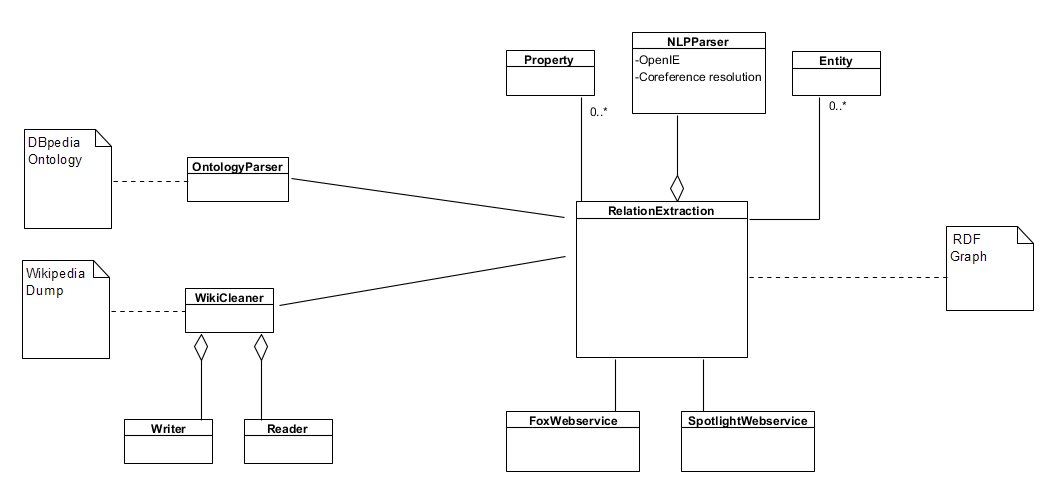
\includegraphics[width=\textwidth]{architecture.png}
\caption{A quick overview of the architecture of our project.} \label{fig1}
\end{figure}


\section{Preprocessing}
The preprocessing consists of the cleaning of the wikipedia dump and the coreference resolution.
\subsection{Extraction and cleaning of the text from a wikipedia dump}
As the foundation we were provided with a wikipedia dump. This wikipedia dump already came without markup, infoboxes 
or chapter subdivisions. The fact that there are no infoboxes already presented some problems, but more to that during the evaluation and discussion. But there were still some elements that were undesired for the later steps in this process. Such elements include unnecessary URLs, text in parenthesis, whitespace, nullchars and special symbols. We removed the texts passages in parenthesis because the Stanford Core NLP had some problems with these during the binary relation extraction for our own approach later on. The elements were removed under application of some regular expressions. 
\pagebreak

The result is a simple text containing only the letters from the english alphabet, numbers, periods, commas and of course simple spaces. In order to speed up the cleaning process, we used a combination of Reader,Worker and Writer threads. To handle the concurreny we used BlockingQueues from the standard Java libraries. One which the Reader thread uses to pass the read lines to the Worker threads and another one which the Worker threads use to pass the cleaned lines to the Writer thread.


\subsection{Coreference Resolution}
Another step that needs to be taken before the information can be properly extracted is the coreference resolution, so that Spotlight and Fox can also recognize named entities in sentences were previously only a coreference appeared. Therefore we have to replace the pronouns with their representative mention. To actually find this representative mention we used the coref annotator \cite{coref} of the Stanford Core NLP.  

\begin{example} John met Judy in 1960. He married her during his college year.\end{example}

In this sentence we obviously want to replace the he, her and his with their corresponding representative mention.
The result would look like this: 

\begin{example} John met Judy in 1960. John married Judy during John's college year. \end{example}


This example already shows one of the challenges that arise during the coreference resolution. Possesive pronouns have to be detected and handled accordingly. So in this case \textit{his} should not be replaced with \textit{John} but rather with \textit{John's}. To make this distinction we use the dependency parser \cite{parser} of the Stanford Core NLP. Here we take the pronoun in question and then determine if it appears in connection with a possesion modifier relation. If it does, we adjust the representative mention the pronoun will be replaced with accordingly.



\section{Named Entity Recognition}
For this step we use the DBpedia Spotlight web service. We send the text to DBpedia Spotlight and receive a JSON response. The response is then parsed and the found entities and their information is stored in objects of our Entity class. As information we keep the uri, surface form, offset and the types. Since we send more than one sentence at a time to Spotlight we need to keep the offset to map the entities back to their corresponding sentence where they appeared. The surface form we need later on for our own relation extraction where we have to locate the entities inside binary relations. In addition to that we also keep the types because during our own relation extraction we compare these to the range and domain of some properties.





\section{Entity Disambiguation}
The Entity Disambiguation itself is already done by Spotlight and Fox. Spotlight for example has two approaches for this.
After they have located a candidate they take the information next to the surface form as information and try to determine the best match based on that. They also try to weigh words on their ability to actually disambiguate between candidates \cite{disambiguate}. Fox and AGDISTIS \cite{agdistis} were already discussed in the lecture.

\section{Relation Extraction}

\subsection{Using Fox}
\subsection{Own Approach}
After recognizing the entities correctly we need to find the relations between them mentioned in the given Wikipedia dump to finish our knowledge graph. The relation become the edges of the graph.

The type of relation we are most interested in are binary relations, so relations between only two entities an not more. Therefore, we need to find those first. The relations of this type that can be found in our example include:
\begin{example}
First sentence: Obama - be bear on - August 4 1961. (among others)

Second sentence: Obama - graduate from - Havard Law school (among others)\end{example}

Afterwards, we add the relation to our graph. In order to do so, we first look at the subject of the binary relation. In both sentences from our example we recognize "Obama" as the subject with its type including "Person". Then we look at the object of the relation. In the first sentence, we detect that the object contains numbers, which can indicate that the object contains either a date or a number literal. We check whether the object is a date and if it is not, we extract it as a single literal of a fitting number type if it is a number or keep it as a string if the number just happens to be part of a name and therefore not convertable to any other type of literal. In our case, we detect "August" is a month and therefore convert the whole object to the proper dateformat 1961-08-04. In the second sentence, we detect "Hardvard University" as another entity of type EducationalInstitution. Then, in order to be able to map the found relation to the correct property, we look at the predicate of the sentences and check for keywords. In our first sentence, we find "bear" in a relation with "Person" as the domain and xsd:date as range so we search for a property which fits this keyword, domain and range and get dbo:birthDate, while in our second sentence we find the keyword "graduate" with "Person" as domain and " EducationalInstitution" as range and get dbo:almaMater as the fitting property. With these informations, we turned the first and second sentence of our example into the following triples:
\begin{example} First sentence: dbo:Barack\_Obama dbo:birhtDate "1961-08-04".
	
	Second sentence: dbo:Barack\_Obama dbo:almaMater dbo:Havard\_University.\end{example}

These triples can now be properly added to our knowledge graph. After this has been done with all found triples our knowledge graph from the given text is as far completed as the programm is capable to do so.

For this step again we use FOX and Spotlight. We use FOX in "re" mode for entity recognition and relation extraction, however FOX does not recognize many triples and misses too many relations. Therefore we implemented our own method using Spotlight and OpenIE.
We use DBdia Spotlight first for named entity recognition so that we can run our method concurrent to FOX. 

\section{Example}
In the following we will demonstrate the whole process at an example.

\begin{example}
Obama was born on August 4, 1961, at Kapiolani Medical Center for
Women and Children in Honolulu, Hawaii. He graduated from Harvard
University.\end{example}

After the coreference resolution the sentence will look like this: 

\begin{example}
	Obama was born on August 4, 1961, at Kapiolani Medical Center for
	Women and Children in Honolulu, Hawaii. Obama graduated from Harvard
	University.\end{example}

Next we use OpenIE to extract binary relations from the sentences, some of them are listed in the following table.


\begin{table}
		\caption{Shortened version of the binary relations extracted by OpenIE. (only some of the important ones we can actually use)}\label{tab1}
	\begin{center}
		\begin{tabularx}{\textwidth}{@{}|l|l|Y|@{}}
			\hline
			\textbf{Subject} &  \textbf{Predicate} & \textbf{Object}\\
			\hline
			Obama &  be bear on & August 4 1961\\
			Obama &  graduate from & Harvard University\\
			Obama &  be bear at & Kapiolani Medical Center for Women in Honolulu\\
			\hline
		\end{tabularx}
	\end{center}
\end{table}

Then Spotlight will find the following Named Entities.

\begin{example}
\textbf{Obama} was born on August 4, 1961, at \textbf{Kapiolani} Medical Center for
Women and Children in \textbf{Honolulu}, \textbf{Hawaii}. \textbf{Obama} graduated from
\textbf{Harvard University} .\end{example}

Now as already discussed we will try to map the subject, predicate and object to entities, properties and entities or literals. Here we distinguish between entity to literal relation and entity to entity relation.
\pagebreak

\begin{table}
	\caption{Mappings entity to literal relation. For the first binary relation of Table 1.}\label{tab2}
	\begin{center}
		\begin{tabularx}{\textwidth}{@{}|l|l|Y|@{}}
			\hline
			\textbf{Part of binary relation} &  \textbf{Keywords} & \textbf{Mapping}\\
			\hline
			Subject &  Obama & dbr:Barack\_Obama\\
			Predicate &  bear & dbo:birthDate\\
			Object &  August 4 1961  & 1961-08-04\\
			\hline
		\end{tabularx}
	\end{center}
\end{table}

\begin{table}
	\caption{Mappings entity to entity relation. For the third binary relation of Table 1.}\label{tab3}
	\begin{center}
		\begin{tabularx}{\textwidth}{@{}|l|l|Y|@{}}
			\hline
			\textbf{Part of binary relation} &  \textbf{Keywords} & \textbf{Mapping}\\
			\hline
			Subject &  Obama & dbr:Barack\_Obama\\
			Predicate &  graduate & dbo:almaMater\\
			Object &  Harvard University  & dbr:Harvard\_University\\
			\hline
		\end{tabularx}
	\end{center}
\end{table}
So finally we get these two triples and write them to the graph. In this example we could also find the triple with the birth place of Honolulu. 

\section{Evaluation}
\subsection{Runtime}

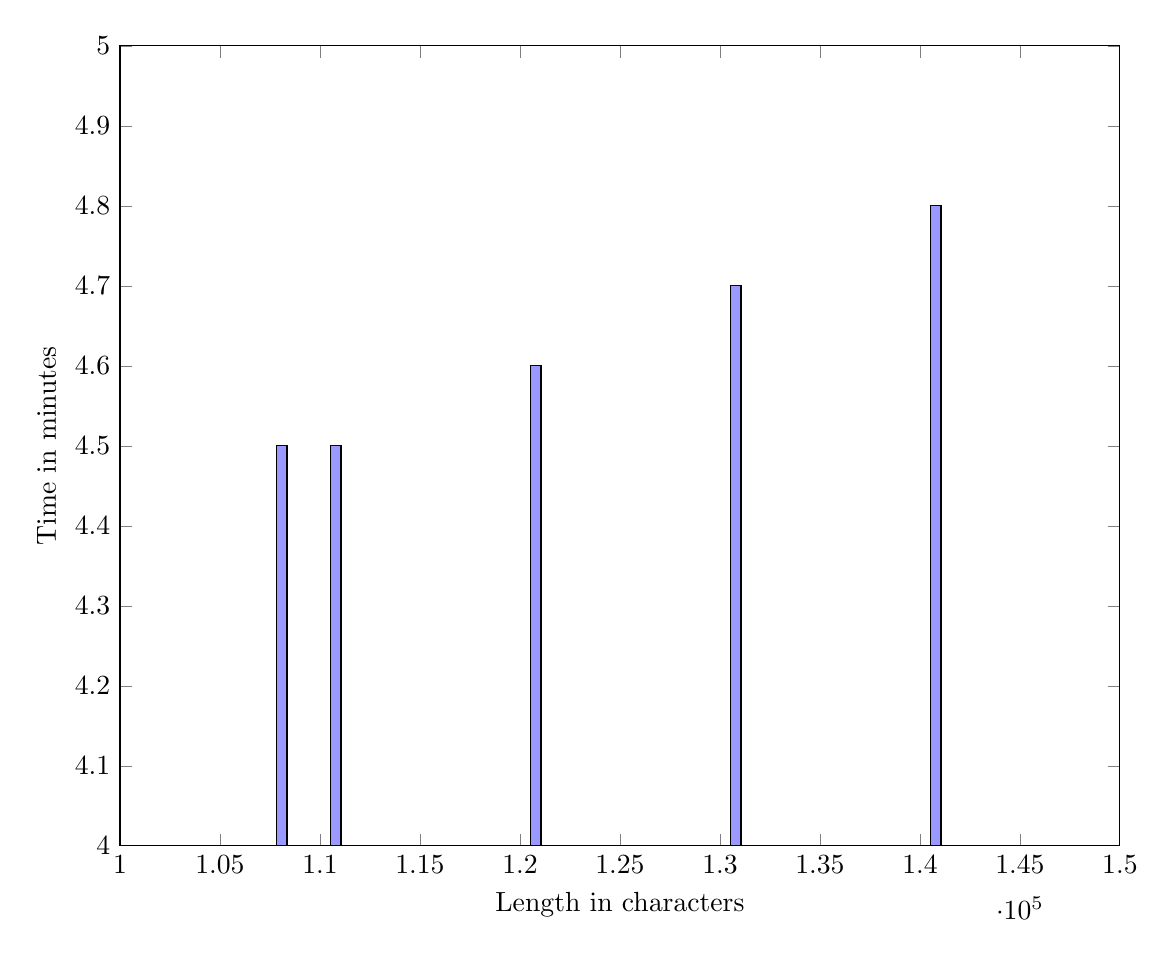
\begin{tikzpicture}
\begin{axis}[%
scale only axis,
width=5in,
height=4in,
xlabel=Length in characters,
ylabel= Time in minutes,
xmin=100000, xmax=150000,
ymin=4, ymax=5,
axis on top]
\addplot[
ybar,
bar width=0.0502874in, 
bar shift=0in,
fill=blue!40,
draw=black] 
plot coordinates{ 
	(108100,4.5) (110800,4.5) (120800,4.6) (130800,4.7) (140800,4.8)
};

\end{axis}
\end{tikzpicture}

\subsection{Correctness}


% ---- Bibliography ----
%
% BibTeX users should specify bibliography style 'splncs04'.
% References will then be sorted and formatted in the correct style.
%

\bibliography{references}
\bibliographystyle{splncs04}
%


\end{document}
